\section{Foundations of Economics}
{
\subsection{Fundamental Problem of Economics}
{
Human beings have many wants and needs. The physical objects they want or need are called 
\emph{goods} (e.g., food, clothing, books), while the non-physical activities are called 
\emph{services} (e.g., education, health care, entertainment).

The study of economics arises because people's needs and wants are unlimited, but the
\emph{resources} needed to satisfy them are limited. Resources are inputs used to produce
goods and services, and for this reason are also known as \emph{factors of production}. Factors 
of production do not exist in abundance; they are \emph{scarce}.
\dfn{Scarcity}{Scarcity is the situation in which available resources, or factors of production, are finite,
whereas wants are infinite. There are not enough resources to produce everything that human beings
need and want.}

As a result of scarcity, choices need to be made. Resource scarcity
forces society to make a choice between available alternatives.
Another important consequence of scarcity is avoiding waste in using
resources. If resources are not used effectively and are wasted,
they will end up producing less. Finally, scarcity gives rise to
\emph{opportunity cost}.
\dfn{Opportunity Cost}{Opportunity cost is defined as the value of the next
best alternative that must be given up or sacrificed in order to obtain something else.}
When a consumer chooses to use her \(\$\)100 to buy
a pair of shoes, she is also choosing not to use this
money to buy books. The foregone books are the opportunity cost.
}

\subsection{Assumptions in Model-Building}
{
Economists primarily make two assumptions when building models:
\begin{enumerate}
    \item Ceteris Paribus
    \item Rational Agents
\end{enumerate}

\dfn{Ceteris Paribus}{A Latin expression that means `other things equal'.
In the context of economics, it is saying that all other things are assumed to be constant or unchanging
in order to study the effect of one independent variable on a dependent variable.}

\dfn{Rational Agents}{Rational economic decision-making. This 
means that individuals are assumed to act in their best self-interest, trying to maximise
(make as large as possible) the satisfaction they expect to receive from their decisions.}
}

\subsection{What is Microeconomics?}
{
\dfn{Microeconomics}{Microeconomics is concerned with the behaviour of
consumers, firms and resource owners, who are the most
important economic decision-makers in a market economy.}
}
}


\newpage


\section{Demand and Supply}
{
\subsection{What is a Market?}
{
It is easiest to understand what a market is and how it works by dividing
individual economic units into two broad groups, according to function,
\emph{buyers} and \emph{sellers}.

Buyers purchase goods and services. Usually, there are two types of buyers:
consumers and firms. Consumers purchase regular goods and service while firms
purchase labor, capital, and raw materials that they use to produce goods and services.

Sellers sell goods and services. Usually, there are three types of sellers: firms,
resource owners, and workers. Firms sell their goods and services, resource owners
rent land or sell mineral resources to firms, and workers sell their labor services.

\dfn{Market}{A market is an arrangement where buyers and sellers meet to
carry out an exchange which determines the price of a product.}
}

\subsection{Competitive and Non-Competitive Markets}
{
A \emph{perfectly competitive market} has many buyers and sellers, so that
no single buyer or seller has any impact on price. Most agricultural markets are
close to being perfectly competitive. This should be contrasted with \emph{market
power} (a.k.a \emph{monopoly power}), which refers to the control that a seller
has over the price of the product they sell. To make analysis easier, we begin
the study of microeconomics by assuming perfectly competitive markets.

Some markets contain many producers but are \emph{non-competitive}; that is, individual firms can
jointly affect the price. The world oil market is one such example. Since the early
1970s, that market has been dominated by the OPEC cartel.
}

\subsection{Demand}
{
\dfn{Demand}{The demand represents how much of a good consumers are \emph{willing} and \emph{able} to buy
at different possible prices in a particular time period.}

There are two keywords in the definition; willing and able. `Willing' means that consumers want to
buy the product. `Able' means they can afford the product. For instance, consider the demand for
Ferraris. You may want to buy a Ferrari, but can you afford it? If not, your desire to buy one
will not show up as demand for Ferraris.

The demand for a product is usually represented by a curve with the possible prices on the \(y\)-axis
and the quantity demanded on the \(x\)-axis.

\begin{figure}[H]
    \centering
    \begin{tikzpicture}[scale=1.25]
        % Axes
        \draw[->] (0,0) -- (5,0) node[right]{Quantity};
        \draw[->] (0,0) -- (0,4) node[above]{Price};

        % Demand curve D
        \draw[thick,blue] (0.5,3.5) to[out=-60,in=150] (4,0.5) node[right] {$D$};

        % P1 line
        \draw[dashed] (0,1.75) node[left]{$P_{1}$} -- (2,1.75);

        % Q1 line
        \draw[dashed] (2,0) node[below]{$Q_{1}$} -- (2,1.75);

        % Intersection point
        \fill (2,1.75) circle (2pt);
    \end{tikzpicture}
    \caption{Demand Curve}
    \label{fig:dcurve1}
\end{figure}

\subsubsection{Why Does the Demand Curve Slope Downward?}
{
There are two explanations for the downward slope of the demand curve:
\begin{enumerate}
    \item Law of Demand
    \item Law of Diminishing Marginal Benefit
\end{enumerate}

\dfn{Law of Demand}{There exists a negative causal relationship between price and quantity demanded.
As the price of a good decreases, the quantity of the good demanded increases, ceteris paribus.}

\dfn{Law of Diminishing Marginal Benefit}{Consumers buy goods because
it provides them with some benefit or satisfaction known as \emph{utility}. The greater the
quantity of a good consumed, the greater the utility. However, the extra benefit
provided by each additional unit increases by smaller and smaller amounts.
The extra benefit that you get from each additional unit of something you buy is called the
\emph{marginal benefit} or \emph{marginal utility} (marginal means extra or additional).
Since each successive unit of the good you consume produces less and less benefit,
you will be willing to buy each extra unit only if it has a lower and lower price.}
}

\subsubsection{Non-Price Determinants of Demand}
{
\begin{figure}[H]
    \centering
    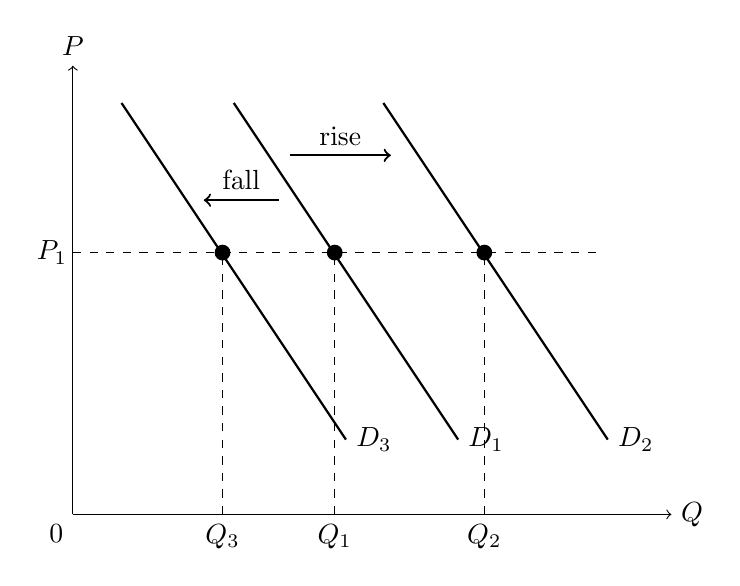
\begin{tikzpicture}[scale=0.95]

    % Axes
    \draw[->] (0,0) -- (8,0) node[right] {$Q$};
    \draw[->] (0,0) -- (0,6) node[above] {$P$};

    % Demand curves
    \draw[thick,black] (0.65,5.5) -- (3.65,1) node[right] {$D_3$};
    \draw[thick,black] (2.15,5.5) -- (5.15,1) node[right] {$D_1$};
    \draw[thick,black] (4.15,5.5) -- (7.15,1) node[right] {$D_2$};

    % Price line P1
    \draw[dashed,black] (0,3.5) -- (7,3.5) node[left=6.6cm] {$P_1$};

    % Intersections with demand curves
    \draw[dashed,black] (2,0) node[below] {$Q_3$} -- (2,3.5);
    \draw[dashed,black] (3.5,0) node[below] {$Q_1$} -- (3.5,3.5);
    \draw[dashed,black] (5.5,0) node[below] {$Q_2$} -- (5.5,3.5);
    \fill (2,3.5) circle (3pt);
    \fill (3.5,3.5) circle (3pt);
    \fill (5.5,3.5) circle (3pt);

    % Arrows indicating shift
    \draw[->,black,thick] (2.75,4.2) -- (1.75,4.2) node[midway,above] {fall};
    \draw[->,black,thick] (2.9,4.8) -- (4.25,4.8) node[midway,above] {rise};

    % Origin
    \node[below left] at (0,0) {0};
    \end{tikzpicture}
    
    \caption{Shift in Demand}
    \label{fig:dcurve2}
\end{figure}

The non-price determinants of demand are factors other than price which influence demand. These
are the factors assumed to be constant by the ceteris paribus assumption in the law of demand.
Changes in the determinants of demand cause shifts in the demand curve; the entire demand
curve moves to the right or left. The factors that cause a shift in the demand curve are:
\begin{multicols}{2}
    \begin{enumerate}
        \item Income (Normal Goods)
        \item Income (Inferior Goods)
        \item Preferences
        \item Price of Substitute Goods
        \item Price of Complementary Goods
        \item Demographic Changes
    \end{enumerate}
\end{multicols}

\dfn{Normal Goods}{A good is a normal good when demand for it increases
in response to an increase in consumer income. Most goods are normal goods.}
\dfn{Inferior Goods}{A good is an inferior good when demand for it decreases
in response to an increase in consumer income. Examples of
inferior goods are second-hand clothes, used cars, and bus tickets.}

\dfn{Substitute Goods}{Goods are substitutes when an increase in
the price of one leads to an increase in the quantity demanded of the other.
Coca-cola and Pepsi are examples of substitute goods.}
\dfn{Complementary Goods}{Goods are complements when an increase in the price of one leads to a decrease
in the quantity demanded of the other. Petroleum and automobiles are
examples of complementary goods.}

\newpage

It is important to distinguish between movements on or along a demand curve, and shifts of a
demand curve. Whenever the price of a good changes, ceteris paribus, it leads to a movement along the demand curve,
this is called \emph{change in quantity demanded}.
By contrast, any change in a non-price determinant
of demand results in a shift in the entire demand curve, this is called a \emph{change in demand}.
To distinguish between these two changes,
different terminology is used. The phrase \emph{change in demand}
refers to shifts in the demand curve, while the phrase \emph{change in the
quantity demanded} refers to movements along the demand curve.
}
}

\subsection{Supply}
{
\dfn{Supply}{The supply represents how much of a good producers are \emph{willing} and \emph{able} to produce at
different possible prices in a particular time period.}

The supply of a product is usually represented by a curve with the possible prices on the \(y\)-axis
and the quantity supplied on the \(x\)-axis.

\begin{figure}[H]
    \centering
    \begin{tikzpicture}[scale=1.25]
        % Axes
        \draw[->] (0,0) -- (5,0) node[right]{Quantity};
        \draw[->] (0,0) -- (0,4) node[above]{Price};

        % Supply curve S
        \draw[thick,red,domain=0:4,samples=200,smooth,variable=\x]
        plot (\x,{(0.1*\x*\x + 0.5*\x)+0.3725});

        % P1 line
        \draw[dashed] (0,1.75) node[left]{$P_{1}$} -- (2,1.75);

        % Q1 line
        \draw[dashed] (2,0) node[below]{$Q_{1}$} -- (2,1.75);

        % Intersection point
        \fill (2,1.75) circle (2pt);
    \end{tikzpicture}
    \caption{Supply Curve}
    \label{fig:scurve1}
\end{figure}

\subsubsection{Why Does the Supply Curve Slope Upward?}
{
Higher prices generally mean that a firm's profits increase, and so the firm faces an incentive
to produce more output. Lower prices mean lower
profitability, and the incentive facing the firm is
to produce less. Therefore, there results a positive
relationship between price and quantity supplied: the
higher the price, the greater the quantity supplied.
}

\subsubsection{Vertical Supply Curve}
{
While it is true that the supply curve generally slopes upward, a few important exceptions
remain wherein the supply curve is vertical.

\begin{figure}[H]
    \centering
    \begin{tikzpicture}[scale=1.25]
        % Axes
        \draw[->] (0,0) -- (5,0) node[right]{Quantity};
        \draw[->] (0,0) -- (0,4) node[above]{Price};

        % Supply curve S
        \draw[black] (2.5,0) -- (2.5,3.75) node[above, right] {$S$};

        % Origin
        \node[below left] at (0,0) {0};
    \end{tikzpicture}
    \caption{Supply Curve}
    \label{fig:scurve2}
\end{figure}

Consider a movie theatre. No matter what happens, the number of people a theatre can accomodate
remains fixed. No matter how high the price, it is not
possible to increase the number of seats in a short period of time. Another example for
this is original antiques and paintings. There is a fixed quantity of the good because there
is no possibility of ever producing more of it.
}

\subsubsection{Non-Price Determinants of Supply}
{
\begin{enumerate}
    \item Cost of Resources
    \item Technology
    \item Taxes
    \begin{itemize}
        \item A \emph{tax} is a mandatory fee levied on individuals and firms by the government
        to improve infrastructure and quality of life
        \item Therefore, the imposition of a new tax (or an increase of an existing tax) is
        equivalent to an increase in production cost
    \end{itemize}

    \item Subsidies
    \begin{itemize}
        \item A \emph{subsidy} is a payment made to a firm by the government, and so has the
        opposite effect of a tax
        \item The introduction of a subsidy (or an increase of an existing subsidy) is equivalent
        to a fall in production costs
    \end{itemize}

    \item Price of Related Goods (Competitive Supply)
    \begin{itemize}
        \item Competitive supply of two products refers to them competing for the use of the same resources,
        and producing more of one means producing less of the other
        \item For example, a farmer, who can grow wheat or corn, chooses to grow wheat. If the price
        of corn increases, the farmer may switch to corn production as this is now more profitable, resulting
        in a fall in wheat supply and a leftward shift of the supply curve
    \end{itemize}

    \item Price of Related Goods (Joint Supply)
    \begin{itemize}
        \item Joint supply of two or more products refers to production of goods that are derived from a single
        product. Hence, it is not possible to produce more of either product without producing more of its source
        \item For example, butter and skimmed milk are both produced from whole milk; petrol and diesel
        are produced from crude oil
    \end{itemize}

    \item Number of Firms
    \item `Shocks' or Unpredictable Events
    \item Producer Expectations
\end{enumerate}

Similar to demand, any change in price produces a change in quantity supplied, shown as a movement on the supply curve.
Any change in a determinant of supply (other than price) produces a change in supply, represented by a
shift of the whole supply curve.
}
}

\subsection{Market Equilibrium}
{
Until now, market demand and market supply have been considered separately to show
the quantities consumers and firms are willing and able to buy and sell at each
price. However, this is not how much they actually buy and sell. Consider the following
\emph{demand and supply schedule} showing various prices and the quantities of
chocolate bars bought and sold at those prices:

\begin{center}
\begin{tabular}{|>{\centering\arraybackslash}m{3cm}|>{\centering\arraybackslash}m{4cm}|>{\centering\arraybackslash}m{4cm}|}
\hline
\rowcolor{lightgray}
\textbf{Price of chocolate bars (\$)} & 
\textbf{Quantity of chocolate bars demanded (per week)} & 
\textbf{Quantity of chocolate bars supplied (per week)} \\
\hline
5 & 4000 & 12000 \\
\hline
4 & 6000 & 10000 \\
\hline
3 & 8000 & 8000 \\
\hline
2 & 10000 & 6000 \\
\hline
1 & 12000 & 4000 \\
\hline
\end{tabular}
\end{center}

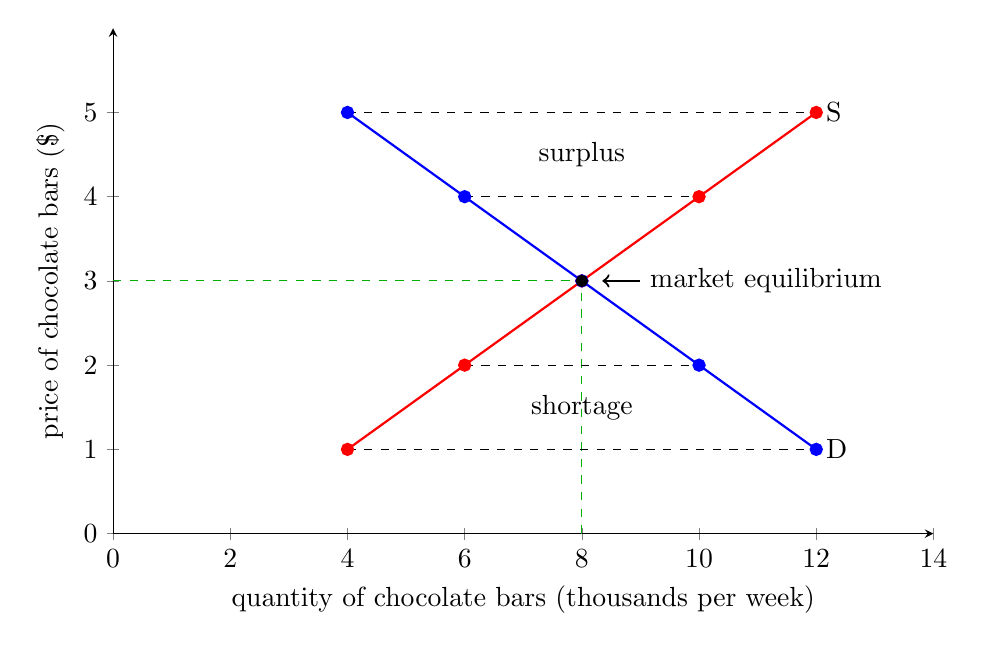
\begin{tikzpicture}
\begin{axis}[
    axis lines=left,
    xlabel={quantity of chocolate bars (thousands per week)},
    ylabel={price of chocolate bars (\$)},
    xmin=0, xmax=14,
    ymin=0, ymax=6,
    xtick={0,2,4,6,8,10,12,14},
    ytick={0,1,2,3,4,5},
    grid=none,
    width=12cm,
    height=8cm,
    enlargelimits=false
]

% Supply curve (red)
\addplot[red, thick, mark=*] coordinates {
    (4,1) (6,2) (8,3) (10,4) (12,5)
};

% Demand curve (blue)
\addplot[blue, thick, mark=*] coordinates {
    (4,5) (6,4) (8,3) (10,2) (12,1)
};

% Market equilibrium point
\addplot[only marks, mark=*, mark size=2pt] coordinates {(8,3)};
\node[right] at (axis cs:9,3) {market equilibrium};

% Equilibrium price (horizontal dashed line)
\draw[dashed, green!70!black] (axis cs:0,3) -- (axis cs:8,3);

% Equilibrium quantity (vertical dashed line)
\draw[dashed, green!70!black] (axis cs:8,0) -- (axis cs:8,3);
\draw[->, thick, black] (axis cs:9,3) -- (axis cs:8.35,3);

% Surplus line
\draw[dashed] (axis cs:4,5) -- (axis cs:12,5);
\draw[dashed] (axis cs:6,4) -- (axis cs:10,4);
\node at (axis cs:8,4.5) {surplus};

% Shortage line
\draw[dashed] (axis cs:4,1) -- (axis cs:12,1);
\draw[dashed] (axis cs:6,2) -- (axis cs:10,2);
\node at (axis cs:8,1.5) {shortage};

% Labels for supply and demand curves
\node[right] at (axis cs:12,5) {S};
\node[right] at (axis cs:12,1) {D};

\end{axis}
\end{tikzpicture}

Here, there are three important observations:
\begin{enumerate}
    \item There is only one price at which the quantity demanded is equal to the quantity supplied: \$3.
    Here, the quantity demanded (\Qd) is 8000 units and quantity supplied (\Qs) is also 8000
    units.
    \item At a higher price, say \$4, quantity supplied (10000 bars) is greater than quantity demanded
    (6000 bars). Hence, there is a \emph{surplus} (\emph{excess supply}) of 4000 bars.
    \item At a lower price, say \$2, quantity demanded (10000 bars) is larger than quantity supplied (6000
    bars). Hence, there is a \emph{shortage} (\emph{excess demand}) of 4000 bars.
\end{enumerate}

Suppose that the price is initially \$5. What will happen?
If the price is \$5, then \Qd is 4000 bars while the \Qs is 12000 bars. There is a surplus
of 8000 bars. With unsold output of 8000 bars, producers will lower prices to encourage consumers to buy
more. As the price falls, \Qd becomes larger. Furthermore, there is downward
pressure on the price which falls until \Qd equals \Qs and the surplus
is eliminated. The opposite happens if the price is initially \$1.
The producers notice that the supply is ``quickly'' sold, and so they begin
raising the prices.

It is, therefore, imperative to understand that the existence of a shortage or surplus in
a free market will cause the price to change so that \Qd is equal to \Qs.

\dfn{Market Equilibrium}{\emph{Equilibrium} is a market phenomenon wherein the quantity demanded is equal to the quantity supplied
(\Qd equals \Qs) and there is no tendency for
the price to change. In a \emph{market disequilibrium}, there is excess demand (shortage) or excess supply (surplus),
and the forces of demand and supply cause the price to change until the market reaches equilibrium.}

\subsubsection{Changes in Market Equilibrium}
{
\begin{enumerate}
\item Increase in Demand
    \begin{figure}[H]
        \centering
        \includegraphics[scale=0.71]{DEM1}
        \label{fig:dem1}
    \end{figure}
Initially, the market is in equilibrium at point A. Then, a change in a non-price determinant of demand causes an increase in demand
shifting the demand curve to the right. As demand increases and price remains the same, there is a shift to point B. 
There is excess demand (equal to \(b-a\)) at the current price P\(_1\). Point B is a disequilibrium which causes a shortage,
thus exerting upward pressure on price. Hence, the price increases causing a movement along D\(_\text{2}\) and the excess 
demand is eliminated. Finally, the market reaches equilibrium at point C. At C, there is a higher equilibrium quantity (Q\(_2\)) and
a higher equilibrium price (P\(_2\)).

\item Increase in Supply
    \begin{figure}[H]
        \centering
        \includegraphics[scale=0.71]{SUPP1}
        \label{fig:supp1}
    \end{figure}

\item Decrease in Demand
    \begin{figure}[H]
        \centering
        \includegraphics[scale=0.71]{DEM2}
        \label{fig:dem2}
    \end{figure}

\item Decrease in Supply
    \begin{figure}[H]
        \centering
        \includegraphics[scale=0.71]{SUPP2}
        \label{fig:supp2}
    \end{figure}
\end{enumerate}
}
}

\subsection{Linear Demand and Supply Functions}
{

\subsubsection{Linear Demand Function and Its Graph}
{
A demand function has the form:
\[Q_d = a - bP\]
where \Qd is the quantity demanded, \(a\) is the \emph{\(x\)-intercept}, \(b\) is the
slope, and P is the price.

Note that \(a\) is the \emph{\(x\)-intercept} not the
\emph{\(y\)-intercept} and it represents all the variables that are held
constant under the ceteris paribus assumption, i.e. the non-price determinants
of demand.

The slope is calculated as: \(\Delta Q_d \divisionsymbol \Delta P\).
It's interpretation is that for every 1 unit change in the price (\(P\)), the
quantity demanded (\(Q_d\)) changes by \(b\) units.

Suppose that the demand function \(Q_d = 14 - 2P\) is given. It can be plotted as:
\begin{center}
\begin{tikzpicture}
\begin{axis}[
    axis lines=middle,
    xlabel={$Q$},
    ylabel={$P$},
    xlabel style={at={(axis description cs:1.025,0)}, anchor=west}, % right of x-axis
    ylabel style={at={(axis description cs:0,1.025)}, anchor=south}, % above y-axis
    xmin=0, xmax=16,
    ymin=0, ymax=8,
    xtick={0,2,4,6,8,10,12,14,16},
    ytick={0,1,2,3,4,5,6,7,8},
    width=10cm,
    height=7cm,
    domain=0:16,
    samples=100
]

% Demand curve: P = (10 - Q)/2
\addplot[blue, thick] {(14 - x)/2};
\end{axis}
\node[below left] at (0,0) {0};
\end{tikzpicture}
\end{center}


Now, we can analyse the parameters \(a\) and \(b\). Firstly, \(a\) represents the
non-price determinants of demand. Therefore, if there is a change in any of 
the non-price determinants of demand (\(a\)), then the curve will shift left or
right parallelly.

\begin{figure}[H]
    \centering
    \includegraphics[scale=0.7]{LDF1}
    \caption{Change in \(a\) causing a shift of the demand curve}
\end{figure}

\par\noindent
Finally, \(b\) represents the slope of the demand curve. The demand curve becomes flatter
as the absolute value of \(b\) increases. Why? Shouldn't it become steeper? No. It needs
to be understood that the graph is not of the form \(y = mx + c\), it is of the
form \(x = a - by\). When the absolute value of \(b\) increases from \(b_1\) to \(b_2\), it means that for a 1 unit
change in price, the quantity demanded now changes by \(b_2\) units rather than \(b_1\)
units where \(|b_2| > |b_1|\); \Qd changes by an amount more than before.

Consider the following example where the demand function changes from \(Q_d = 14 - 2P\)
to \(Q_d = 14 - 4P\):
\begin{figure}[H]
    \centering
    \includegraphics[scale=0.7]{LDF2}
    \caption{Change in \(b\) causing a change in the slope of the demand curve}
\end{figure}
}

\subsubsection{Linear Supply Function and Its Graph}
{
The supply function has the form:
\[Q_s = c - dP\]
where \Qs is the quantity supplied, \(c\) is the \emph{\(x\)-intercept}, \(d\) is the
slope, and P is the price.

Suppose the supply function \(Q_s = 2 + 2P\) is given. It can be plotted as:
\begin{center}
\begin{tikzpicture}
\begin{axis}[
    axis lines=middle,
    xlabel={$Q$},
    ylabel={$P$},
    xlabel style={at={(axis description cs:1.025,0)}, anchor=west}, % right of x-axis
    ylabel style={at={(axis description cs:0,1.025)}, anchor=south}, % above y-axis
    xmin=0, xmax=16,
    ymin=0, ymax=8,
    xtick={0,2,4,6,8,10,12,14,16},
    ytick={0,1,2,3,4,5,6,7,8},
    width=8cm,
    height=6cm,
    domain=0:16,
    samples=100
]

% Demand curve: P = (10 - Q)/2
\addplot[red, thick] {(x-2)/2};
\end{axis}
\node[below left] at (0,0) {0};
\end{tikzpicture}
\end{center}

Here, the parameters \(c\) and \(d\) represent the same things as \(a\) and \(b\) in the
demand function. Firstly, \(c\) is the \emph{\(x\)-intercept} and represents all of the
non-price determinants of supply. If there is a change in any of the non-price determinants
of supply, then \(c\) changes and this causes a shift of the supply curve left or right
parallelly.

\begin{figure}[H]
    \centering
    \includegraphics[scale=0.65]{LSF1}
    \caption{Change in \(c\) causing a shift of the supply curve}
\end{figure}

\par\noindent
Then, \(d\) is the slope of the supply curve. The supply curve becomes flatter
as the absolute value of \(d\) increases. Why? Shouldn't it become steeper? No. It needs
to be understood that the graph is not of the form \(y = mx + c\), it is of the
form \(x = a - by\). When the absolute value of \(d\) increases from \(d_1\) to \(d_2\), it means that for a 1 unit
change in price, the quantity demanded now changes by \(d_2\) units rather than \(d_1\)
units where \(|d_2| > |d_1|\); \Qs changes by an amount more than before for the same
change in price.

\begin{figure}[H]
    \centering
    \includegraphics[scale=0.7]{LSF2}
    \caption{Change in \(d\) causing a change in the slope of the supply curve}
\end{figure}
}

\subsubsection{Market Equilibrium}
{
The demand and supply functions can be combined to find market equilibrium:
\[\begin{aligned}
Q_d &= 14 - 2P \\
Q_s &= 2 + 2P \\
\end{aligned}\]
\[\text{Equilibrium Condition: } \; Q_d = Q_s\]
\[14-2P = 2+2P \Rightarrow 4P = 12 \Rightarrow P^* = 3\]
\[Q^* = 14-2(3) = 2+2(3) \Rightarrow Q^* = 8\]
}
}
}